\documentclass[11pt, letterpaper]{article}
\usepackage[utf8]{inputenc}
\usepackage{graphicx}
\usepackage{amssymb}
\graphicspath{{images/}}
\title{AI1110 Assignment 1}
\author{Abhinav Yadav, cs21btech11002}

\begin{document}
    \maketitle
    \section*{Q11 (b)}
    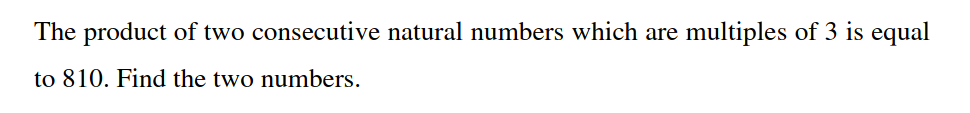
\includegraphics[width=\textwidth]{q11_b.png}
    \section*{Solution}
    Let the two consecutive natural numbers which are multiples of $3$ be $3n$ and $3n+3$
    \hspace{5pt} $\exists \hspace{2pt} n \in \mathbb{N}$
    \newline
    \textbf{According to the question:}\newline
    $\hspace*{12pt} 3n(3n+3) = 810$\newline
    $\Rightarrow 9n(n+1)=810$\newline
    $\Rightarrow n(n+1)=90$\newline
    $\Rightarrow n^2+n-90=0$\newline
    $\Rightarrow (n+10)(n-9)=0$\newline
    $\Rightarrow n=-10 \hspace{15pt} or \hspace{15pt} n=9$\newline
    \hspace*{11pt} discarding $n=-10$ as $n \in \mathbb{N}$\newline
    $\Rightarrow n=9$\newline
    $\Rightarrow 3n=27$\newline
    $\Rightarrow 3n+3=30$\newline
    The two numbers are:\newline
    \begin{tabular}{|c|}
        \hline
            $27, 30$\\
        \hline
    \end{tabular}\newline\newline
    The output of the program used to find and verify these numbers is:\newline
    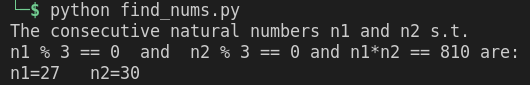
\includegraphics[width=0.9\textwidth]{output.png}

\end{document}